%%%%%%%%%%%%%%%%%%%%%%%%%%%%%%%%%%%%%%%%%%%%%%%%%%%%%%%%%%%%%%%%%%%
% Background
% Team:
% Wolverine
% Members: 
% Dexter Chen, Eric Chang, Eric Lee, Jacky Wu, Karthick Mani, Kenvin Lo, Yu-cheng Chen
% Relative files:
% Main.tex, Background_Wolverine.tex, Library.bib, Wolverine_Background_Chart_1.png
% Note: 
% Do not compile this file compile Main.tex to get the pdf file instead.
%%%%%%%%%%%%%%%%%%%%%%%%%%%%%%%%%%%%%%%%%%%%%%%%%%%%%%%%%%%%%%%%%%%
	
\subsection{Information retrieval on existing database}
\textit{\footnotesize Author:Dexter Chen, Eric Chang, Eric Lee, Jacky Wu, Karthick Mani, Kenvin Lo, Yu-cheng Chen.}\\

We live in the time where technologies evolve beyond our imagination.
Information growth in a exponential rate according to \cite{Tague1981}, thus we can't rely on the old fashion ways to find data we want. 
We need new information retrieval methods to handle such a big amount of data systematically.
But most of the information retrieval methods such as search engine can't really search everything on the web. 
They can only search the data that has been captured into the database according to \cite{Grehan2002}. 
Thus, we need to create a database to store these data and automatically update them frequently.

There are several online libraries currently available for us to get the academic articles or periodicals we need.
And they can be roughly divided into three groups according to the way they store articles base on the division used by National Taiwan University Library.

\paragraph{Index libraries}

	These kind of libraries stores the index and abstract of the articles.
	They don't provide the full-text documents directly, but may give the linkage to the publisher websites of articles.
	And they can be categorized by the type of articles they include.
	
	\begin{itemize}
		
		\item\textbf{Comprehensive topics}\\Libraries such as Web of Science, Scopus...
		\item\textbf{Specialized topics}\\Libraries such as Compendex, BIOSIS Previews, PubMed, MEDline...
		
	\end{itemize}
	
\paragraph{Publisher libraries}

	These libraries are created by the publishers themselves, so they provide the newest and complete documents directly.
	And can also be categorize by the type of articles they include.
	
	\begin{itemize}
		
		\item\textbf{Comprehensive topics}\\Libraries such as Science Direct, Springer Link, Wiley Online Library...
		\item\textbf{Specialized topics}\\Libraries such as Nature.com, Emerald Management Xtra, IEEE Xplore...
		
	\end{itemize}
	
\paragraph{Aggregator libraries}

	These libraries do not publish the articles by themselves, but they still sometimes provide the full-text articles to the user.
	The way they do this is to negotiate with some of the publisher libraries and get the authorization of the articles.
	Libraries such as EBSCOhost, ProQuest, JSTOR...

The comparison between three kinds of library can be found on Figure \ref{WBC1}. 
On the next section we'll discuss about more details about 
some of the existing libraries.

\subsubsection{Introduction to several libraries }\todo{Consider to change the title.}

\begin{enumerate}
	
	\item\textbf{PubMed}
	\setlength{\parindent}{1em}
	 PMC (PubMed Central) is launched in 2000.
	 PubMed citations often include links to the full-text article on the publishers' Web sites or in PMC and the Bookshelf.
	 PubMed is a free library which is used for searching reference papers and abstracts related to the biomedical topics.
	 The largest subset of PubMed is MEDLINE, which is a bibliographic database containing life sciences and biomedical information.
	 Both of them are built by National Library of Medicine.You may limit your search to MEDLINE only in PubMed.
	 
	 A strong feature of PubMed is its ability to link MeSH(Medical Subject Headings) terms automatically. 
	 It is useful for people who want to find the medical articles. 
     Simple searches on PubMed can be carried out by entering tje key words of a subject into PubMed's search window.
     PubMed translates this initial search formulation and automatically adds field names.
	 Like several libraries, one can find the specific result he desires by addding relevant MeSH terms, synonyms and Boolean operators.
	 
	 The design philosophy of PubMed is based on full-text XML files, which are readable by both the machines, humans and moreover technology independent.
	 PubMed is classified into Index libraries, which is the prime reason that it is not able to provide full text in some papers.
	 For the type of database used by PubMed is Microsoft SQL server, which is a relational database to store all of 
	 the archives such as XML, images, PDF files supplementary, etc. \todo{Good that you start by describing what it is and then tell how it is built.}	 
	  
		
	\item\textbf{IEEE Xplore}
	\setlength{\parindent}{1em}
	
	The IEEE is an acronym for Institute of Electrical and Electronics Engineers, which is one of the leading standard organizations in the world 
	It is one of the most professional organization devoted to advancing technology for the benefit of humanity.
	There are more than 420,000 IEEE members in over 160 countries.
	And IEEE Xplore is a scholarly research library formerly known as IEEE/IET Electronic Library (IEL).
	The articles covered by IEEE Xplore are mainly from the Institute of Electrical and Electronics Engineers (IEEE) and the Institution of Engineering and Technology.
	More than 3.5-million full-text documents in the field of electrical, engineering, computer science and electronics are provided in this library. 
	
	There are many features in IEEE. IEEE can rank the articles according to their click through rates or download times. 
    Once an articles is updated by the author, those who set research alert on it will receive a notification through email by IEEE.
    However, some of the features are available for members only.
    Many enterprises and schools are the members of IEEE.

	
	The front and user interface of IEEE library present the information on the screen, 
	including the latest Angular, Jquery, HTML 5, CSS, etc.\todo{You mean it is implemented using these techniques. Please don't use etc. when you describe how something is built and do it in this context.} 
	Most of the HTML for PDF, either it is for journal (conference) articles or standards get dynamic transformations real time and served through MarkLogic.
	Endeca, which is an Oracle product powers Xplore searches, is used in the search layer.
	All PDF files are fed through Endeca system.
	Endeca servers will provide the matching documents and Xplore platform will presents it on the screen to the user.
	And all the content is stored in oracle metadata which will be consumed by Endeca, MarkLogic Authentication, and Authorization services.
	
	\item\textbf{EBSCOhost}
	\setlength{\parindent}{1em}

	EBSCOhost is a popular reference which authorizes users to gain a great many full-text articles from proprietary databases.
	EBSCO Information Services, headquartered in Ipswich, Massachusetts, 
    which is a division of EBSCO Industries Inc., 
    the third largest private company in Birmingham, Alabama, with annual sales of nearly $2$ billion according to the BBJ's 2013 Book of Lists.

    EBSCO offers library resources to customers in academic, medical, K–12,  
    public library, law, corporate, and government markets. 
	Its products include EBSCONET, a complete e-resource management system,
    and EBSCOhost, which supplies a fee-based online research 
    service with 375 full-text databases, a collection
    of 600,000-plus ebooks, subject indexes, point-of-care 
    medical references, and an array of historical digital archives.

    In 2010, EBSCO introduced its EBSCO Discovery Service (EDS) to institutions,
    which allows searches of a portfolio of journals and magazines

	
	\item\textbf{Comparison Xplore}
	\setlength{\parindent}{1em}
	
	PubMed is a free library which contains many databases, like Medline, PreMedline and Publisher Supplied Citations.
    Medline is the largest subset of PubMed.
    One can also access MEDLINE through EBSCOhost.  
    EBSCOhost promises a large number of databases. 
	Many of them, such as MEDLINE and EconLit, are licensed from web content vendors.
    Others, such as Criminal Justice Abstracts, MasterFILE, are compiled by EBSCO itself.

    However, in contrast to other two libraries, the advanced search of PubMed is weak. 
    It do not show citation times or further information.
    And the only database which does not provide full-text documents is PubMed. 

    The documents in PubMed are almost related to the biomedical topics.
    IEEE contains more than one third documents in the field of electrical, engineering, computer science and electronics.
    And the articles of EBSCOhost comprises many fields, like business, education, laws, medical, computer science, and so on.

    Each library has its own features. PubMed can link the MeSH. EBSCOhost can search the videos or photos concerned with the key words you enter. 
    IEEE has many features the other two databases don’t have, like “top downloads list”, “top search terms” and “custom setting” mentioned above.

    

\end{enumerate}

\todo[inline]{You need to add at least one library example of each library type, since you started with different types. Otherwise you could have focused on one type and motivated the focus. For the libraries containing articles you should add several since you are building one. You should also discuss the database techniques, including alternative ones to the used ones, such as MongoDB, Hadoop, etc. Try to compare features.}

\begin{figure*}[htb]
	\begin{center}
		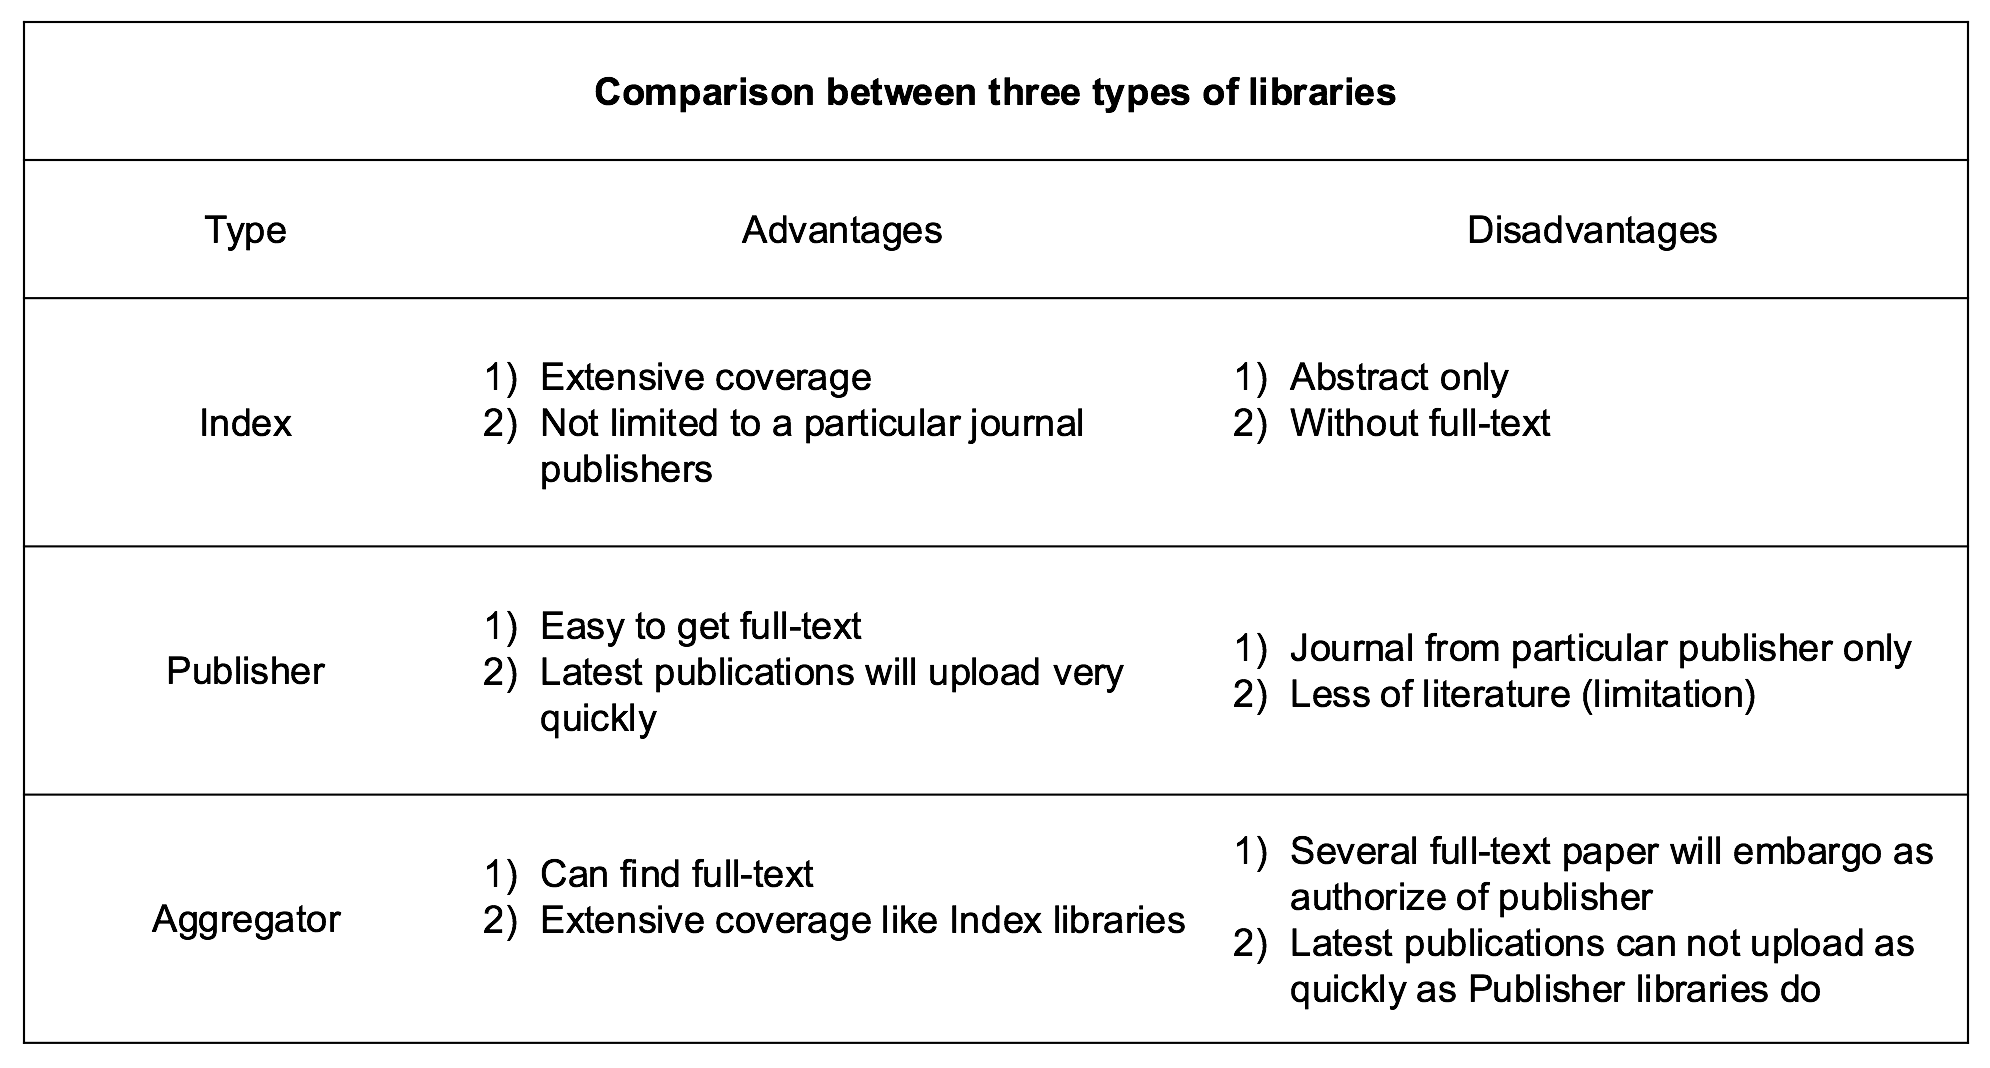
\includegraphics[width=0.8\textwidth]{Wolverine_Background_Chart_1}
	\end{center}
	\caption{Comparison between three types of libraries.\label{WBC1}}
\end{figure*}
\newpage
